\documentclass[landscape]{article}
\usepackage{tikz}
\usepackage{geometry}
\usetikzlibrary{positioning, shapes.geometric, patterns}

% Adjust the page layout with the geometry package
\geometry{left=3cm, right=3cm, top=3cm, bottom=3cm}

\begin{document}
\begin{figure}
    \centering
    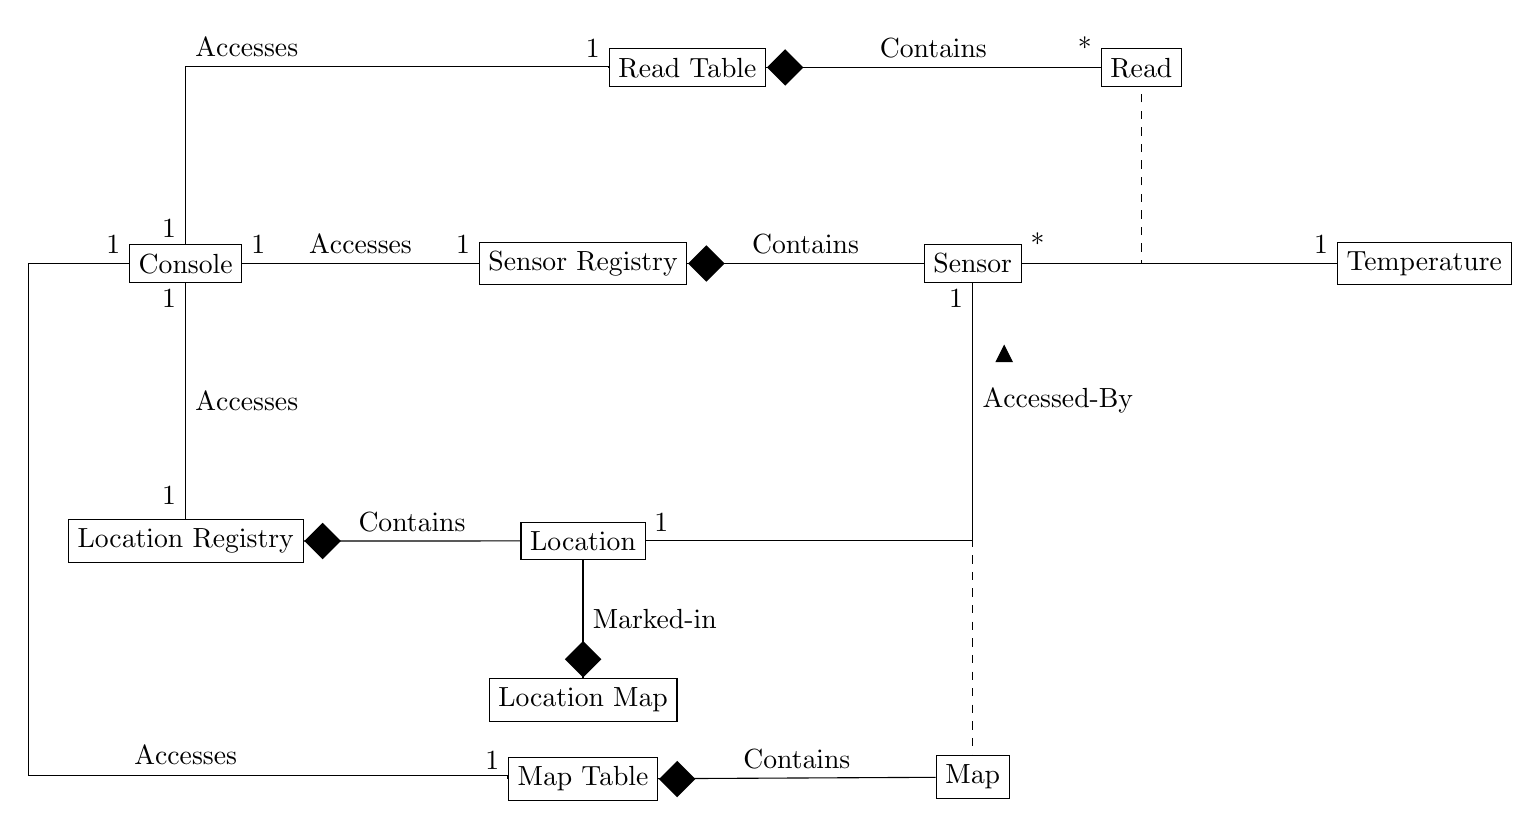
\begin{tikzpicture}[node distance=3cm]
        %-----Entities-----
        
        % Console Entity
        \node[rectangle, draw] (console) {Console};

        % Location Registry Entity
        \node[rectangle, draw, below=of console] (lreg) {Location Registry};

        % Sensor Registry Entity
        \node[rectangle, draw, right=of console] (sreg) {Sensor Registry};

        % Sensor Entity
        \node[rectangle, draw, right=of sreg] (sensor) {Sensor};

        % Location Entity
        \node[rectangle, draw, below=of sreg] (loc) {Location};
        
		% Location Map Entity
        \node[rectangle, draw, below=1.5cm of loc] (locmap) {Location Map};
        
        % Map Entity
        \node[rectangle, draw, below=6cm of sensor] (map) {Map};
        
        % Map Table Entity
        \node[rectangle, draw, below=2.5cm of loc] (mapt) {Map Table};
        
        % Read Entity
        \node[rectangle, draw, above right=2cm and 1cm of sensor] (read) {Read};
        
        % Read Table Entity
        \node[rectangle, draw, above left=2cm and 2cm of sensor] (readt) {Read Table};
        
        % Temperature Entity
        \node[rectangle, draw, right=4cm of sensor] (temp) {Temperature};
        
        %-----Associations and Cardinality-----
        
 		% filled aggregate diamond
        \node[diamond, fill=black, anchor=west, minimum size=10pt] at (mapt.east) {};
        
        % Connect Map Table to Map
        \draw[-] (mapt) -- (map) node[midway, above] {Contains} node[right=0.2cm of mapt, above=0.2cm of mapt.east]{} node[left=0.2cm of map, above]{};
        
        % Connect Read Table to Read
        \node[diamond, fill=black, anchor=west, minimum size=10pt] at (readt.east) {};
        
        \draw[-] (readt) -- (read) node[midway, above] {Contains} node[right=0.2cm of readt, above=0.2cm of readt.east]{} node[left=0.2cm of read, above]{*};
        
        % Connect Console to Map Table
        \draw[-] (console.west)  -- (-2, 0) -| (-2, -6.5) -| (mapt.west) node[left=0.2cm of console,above]{1} node[below=5.75cm of console]{Accesses} node[left=0.2cm of mapt,above]{1};
        
        % Connect Console to Read Table
        \draw[-] (console.north)  -- (0, 2.5) -| (readt.west) node[above=0.2cm of console,left] {1} node[above=2.5cm of console, right] {Accesses} node[left=0.2cm of readt,above]{1};
        
        % Connect Console to Location Registry
        \draw[-] (console) -- (lreg) node[midway, right] {Accesses} node[below=0.2cm of console,left]{1} node[below=2.7cm of console,left]{1};
        
        % Connect Console to Sensor Registry
        \draw[-] (console) -- (sreg) node[midway, above] {Accesses}node[right=0.2cm of console,above]{1} node[left=0.2cm of sreg,above]{1};
         
        % filled black aggregate diamond
        \node[diamond, fill=black, anchor=west, minimum size=10pt] at (sreg.east) {};
        
        % Connect Sensor Registry to Sensor
        \draw[-] (sreg) -- (sensor) node[midway, above] {Contains} node[right=0.2cm of sreg, above]{} node[left=0.2cm of sensor, above]{};

        % Connect Sensor to Temperature 
        \draw[-] (sensor) -- (temp) node[midway, above] {} node[right=0.2cm of sensor,above]{*} node[left=0.2cm of temp,above]{1};
        
        
        
        % Connect Location Registry to Location 
        \node[diamond, fill=black, anchor=west, minimum size=10pt] at (lreg.east) {};
        
         \draw[-] (lreg) -- (loc) node[midway, above] {Contains} node[right=0.2cm of lreg, above=0.2cm of lreg.east]{} node[left=0.2cm of loc, above]{};

        % Connect Location to Sensor 
        \draw[-] (loc) -| (sensor) node[midway, xshift=-1cm, yshift=2cm] {}node[below=0.2cm of sensor, left]{1} node[below=1.5cm of sensor, right]{Accessed-By}  node[right=0.2cm of loc,above]{1};
        
        % Arrow direction between Location and Sensor
        \draw[black, fill=black] (sensor.south) ++(0.3,-1) -- ++(0.2,0) -- ++(-0.1,0.2) -- cycle;
        
        % Connect Location to Location Map
        \node[diamond, fill=black, anchor=south, minimum size=10pt] at (locmap.north) {};
        \draw[-] (loc) -- (locmap) node[midway, right] {Marked-in};


        %-----Associative Entities-----
        \draw[dashed] (sensor.south) ++(0,-3.25) -- (map.north);
        
        \draw[dashed] (sensor.east) ++(2,0) -| (read.south);	

    \end{tikzpicture}
    \caption{Domain Model for Sensor System}
\end{figure}
\end{document}
